\appendix

\section{Details for \Cref{sec:phenomenology}}

\subsection{GRPO Training Details}
\label{app:grpo_details}

\paragraph{Base Model.}
We initialize GRPO training from Qwen3-4B-Base.

\paragraph{Training Dataset.}
We use the processed DAPO-Math-17K dataset for GRPO training. Specifically, each question is augmented with the following instruction:
\begin{tcolorbox}[title=\textbf{GRPO dataset template}, colback=CornflowerBlue!20, colframe=CornflowerBlue!90!Black]
\small
\{Question\} Please reason step by step, and put your final answer within \textbackslash boxed\{\}.
\end{tcolorbox}

\paragraph{Training and Evaluation Settings.}
We train the teacher model using GRPO. During training, we sample $n=8$ responses for each prompt. The maximum prompt length and maximum response length are set to 1,024 and 7,168 tokens, respectively. Training is conducted for one epoch on 8 A800 80G GPUs with a learning rate of $1\times10^{-6}$. We set both the student sampling temperature and the teacher temperature to 1.0, use a repetition penalty of 1.0, disable KL regularization, and adopt \texttt{token-mean} loss aggregation. The main hyperparameters are summarized in \Cref{tab:grpo_hparams}.

\begin{table}[!h]
\centering
\caption{Training hyperparameters of GRPO for Qwen3-4B-Base-GRPO.}
\label{tab:grpo_hparams}
\begin{tabular}{ll}
\toprule
\textbf{Hyper-parameter} & \textbf{Value} \\
\midrule
Base model & Qwen3-4B-Base \\
RL algorithm & GRPO \\
Training epochs & 1 \\
Train batch size & 64 \\
Micro batch size & 64 \\
Rollout $n$ & 8 \\
Maximum prompt length & 1,024 \\
Maximum response length & 7,168 \\
Validation max response length & 31,744 \\
Learning rate & $1 \times 10^{-6}$ \\
Temperature & 1.0 \\
Top-$p$ & 1.0 \\
KL regularization & 0.0 \\
Loss aggregation & \texttt{token-mean} \\
KL Coefficient & 0.0\\
\bottomrule
\end{tabular}
\end{table}

\subsection{Experimental Setup}
\label{app:experimental_setup}

Unless otherwise noted, all experiments use the default OPD hyperparameters listed in Table~\ref{tab:train_hparams_script}.

\begin{table}[t]
\centering
\caption{\textbf{Default hyperparameters for OPD.}}
\label{tab:train_hparams_script}

\begin{tabular}{lc}
\toprule
\textbf{Item} & \textbf{Value} \\
\midrule
Training temperature & 1.0 \\
Global batch size & 64 \\
Mini batch size & 64 \\
Rollout number & 4 \\
LogProb top-$K$ & 16 \\
Top-$K$ strategy & Student Top-$K$ \\
Top-$p$ & 1.0 \\
Max prompt length & 1024 \\
Max response length & 7168 \\
Learning rate & 1e-6 \\
Epoch & 1 \\
KL Coefficient & 0.0\\
\bottomrule
\end{tabular}
\end{table}

\subsection{Benchmark-wise breakdown of thinking-pattern compatibility}
\label{app:thinking_pattern_breakdown}

To further unpack the averaged result in \Cref{fig:thinking_pattern_compatibility}, \Cref{fig:thinking_pattern_compatibility_breakdown} presents a benchmark-wise breakdown.
The advantage of distillation from Qwen3-4B-Base-GRPO is broadly consistent across datasets rather than being driven by a single benchmark.
The gap is more pronounced on AMC 2023 and AIME 2024, and smaller but still generally present on AIME 2025.
This per-benchmark view supports the interpretation that better early-stage thinking-pattern compatibility leads to better downstream distillation performance, and the loss from an early mismatch is not fully recovered later in training.

\begin{figure*}[t]
    \centering
    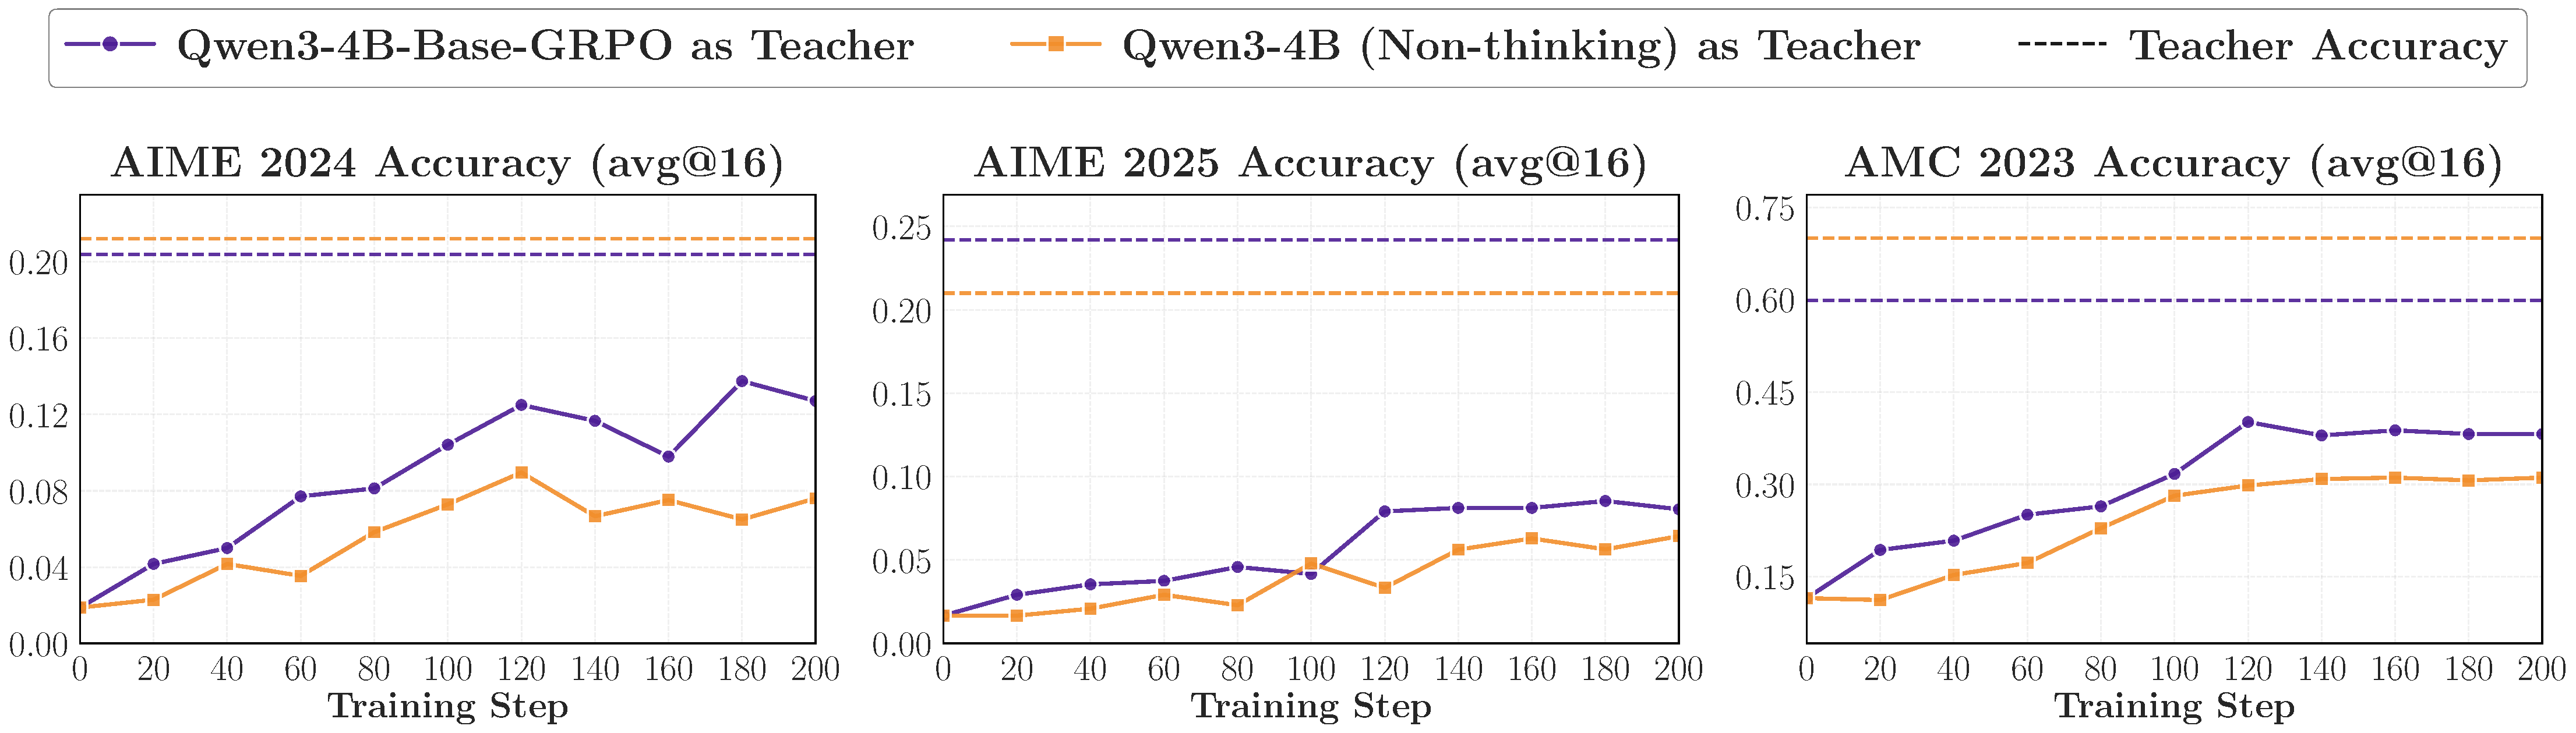
\includegraphics[width=\textwidth]{Figures/3.1/3_1_metrics_benchmarks.pdf}
    \caption{Benchmark-wise breakdown of the average validation accuracy shown in \Cref{fig:thinking_pattern_compatibility}. We report results on AIME 2024, AIME 2025, and AMC 2023 separately. Distillation from Qwen3-4B-Base-GRPO consistently matches or outperforms distillation from Qwen3-4B (Non-thinking) across the three benchmarks.}
    \label{fig:thinking_pattern_compatibility_breakdown}
\end{figure*}

\section{Details for \Cref{sec:mechanism}}

\subsection{Additional Analysis of Token Overlap Mass}
\label{app:overlap_mass}

To quantify how much probability mass each model assigns to the overlap top-$k$ region, we define:
\begin{equation}
\mathcal{M}_{\text{overlap-mass}}^{(p)}
=
\mathbb{E}_{t}\left[
  \sum_{v \in S_t^{(p)} \cap S_t^{(q)}} p_t(v)
\right],
\label{eq:metric_student_overlap_mass}
\end{equation}
and
\begin{equation}
\mathcal{M}_{\text{overlap-mass}}^{(q)}
=
\mathbb{E}_{t}\left[
  \sum_{v \in S_t^{(p)} \cap S_t^{(q)}} q_t(v)
\right],
\label{eq:metric_teacher_overlap_mass}
\end{equation}
which measure the fraction of total probability mass that the student and teacher, respectively, assign to the shared tokens in their top-$k$ sets. In our experiments, the overlap tokens carry $97\%$--$99\%$ of the total probability mass for both models throughout training, as shown in \Cref{fig:overlap-mass}.

\begin{figure}[t]
    \centering
    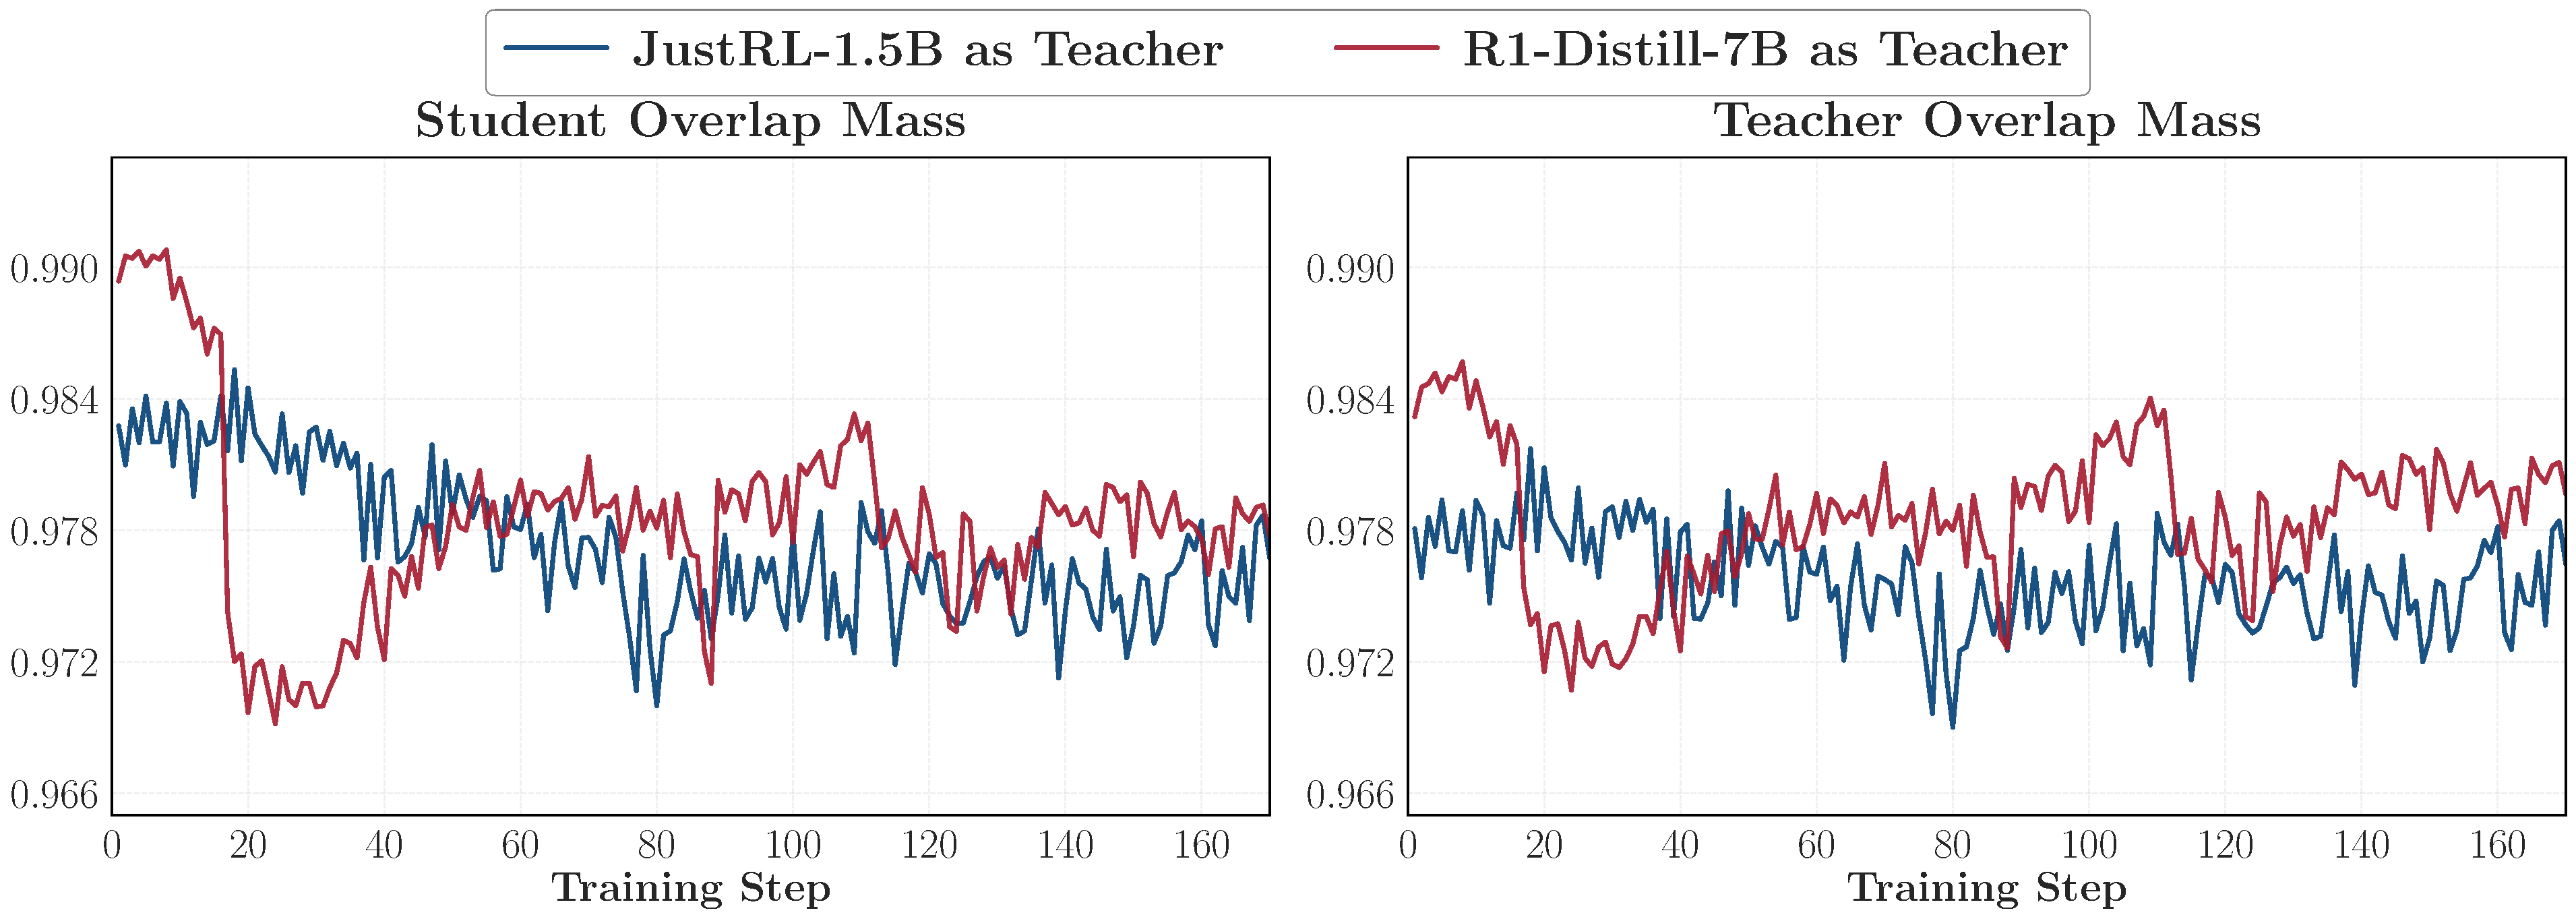
\includegraphics[width=\linewidth]{Figures/appendix/appendix_sum_p.pdf}
    \caption{
    Probability mass assigned to overlap tokens during training.
    For both the student and teacher distributions, the overlap tokens consistently account for roughly 97\%--99\% of the total probability mass, indicating that the overlap is not only increasing at the set level but also dominates the probability distribution.
    }
    \label{fig:overlap-mass}
\end{figure}

\subsection{Auxiliary Optimization Dynamics}
\label{app:auxiliary_dynamics}

To complement the analysis in \Cref{sec:alignment_high_prob}, we report several additional optimization diagnostics for the same contrastive setting. Throughout this appendix, we fix the student to R1-Distill-1.5B and compare two teachers under the same Student Top-$k$ OPD training recipe: JustRL-1.5B, which yields a successful run, and R1-Distill-7B, which yields a failing run under otherwise matched conditions. These diagnostics are not intended as primary evidence; rather, they provide a complementary view of how the optimization signal differs between successful and failing OPD.

\begin{figure*}[t]
    \centering
    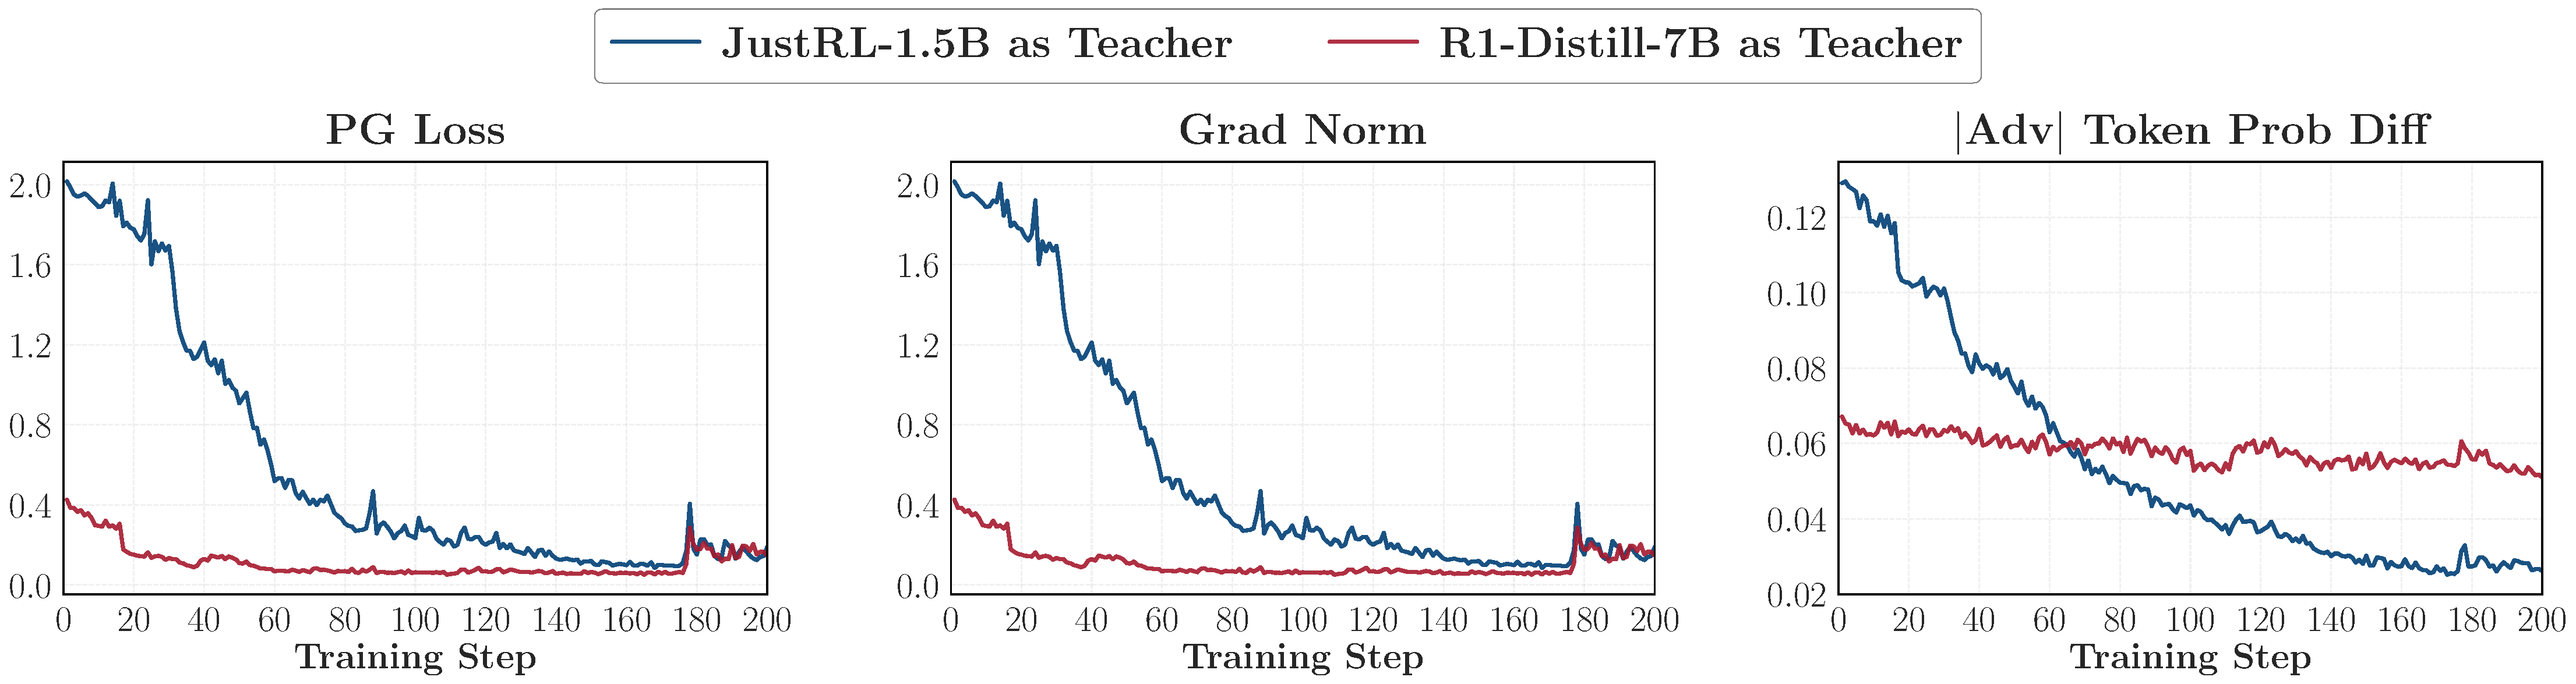
\includegraphics[width=\textwidth]{Figures/appendix/auxiliary_dynamics.pdf}
    \caption{
    Auxiliary optimization diagnostics for the contrastive OPD setting in \Cref{sec:alignment_high_prob}, using R1-Distill-1.5B as the student and comparing JustRL-1.5B against R1-Distill-7B as the teacher. 
    \textbf{Left:} batch-averaged OPD training loss (\textit{PG Loss}) over training. 
    \textbf{Middle:} gradient norm over training. 
    \textbf{Right:} probability difference $p_t(v)-q_t(v)$ measured on the token with the largest absolute advantage. 
    The successful run exhibits a large reduction in optimization loss, sustained gradient magnitude, and a steady decrease in extreme-token probability mismatch. By contrast, the failing run starts with and maintains much weaker gradients, and its extreme-token probability discrepancy remains noticeably larger throughout training.
    }
    \label{fig:auxiliary_dynamics}
\end{figure*}

\paragraph{Diagnostics.}
We monitor three additional quantities. The first is the batch-averaged OPD training loss, denoted as \emph{PG Loss} in \Cref{fig:auxiliary_dynamics}. The second is the gradient norm, which measures the overall magnitude of the update signal reaching the student. The third is the probability difference $p_t(v)-q_t(v)$ on the token with the largest absolute advantage, which tracks whether the student can reduce the most pronounced local disagreement with the teacher on the tokens that carry the strongest optimization signal. Together, these metrics help distinguish between successful and failing OPD: in the former, the student receives a usable signal and progressively reduces mismatch, whereas in the latter, the signal is too weak or too poorly aligned to drive substantial improvement.

\paragraph{Results.}
The trends in \Cref{fig:auxiliary_dynamics} are consistent with the main conclusion of \Cref{sec:alignment_high_prob}. First, the successful run with JustRL-1.5B shows a pronounced reduction in training loss over the course of optimization. Starting from a much larger initial mismatch, the loss decreases steadily for most of training before flattening at a low value. By contrast, the failing run with R1-Distill-7B begins with a much smaller loss and changes only modestly thereafter. This pattern suggests that the smaller loss in the failing run does not indicate better optimization. Rather, it reflects a weak teacher-induced training signal from the outset, which remains too small to drive substantial policy improvement.

Second, the gradient norm shows an even clearer separation between the two runs. In the successful run, the gradient norm is initially large and remains substantial through a long portion of training, indicating that the student continues to receive a meaningful corrective signal. In the failing run, the gradient norm is consistently much smaller, with only limited variation over time. Thus, even though optimization proceeds under the same algorithm and training budget, the student trained against R1-Distill-7B experiences a much weaker update signal. This observation is consistent with the finding that failure is associated with poor alignment on high-probability tokens: when the student does not meaningfully enter the teacher-supported region, the resulting gradients remain weak.

Third, the right panel shows that the successful run steadily reduces the probability discrepancy on the token with the largest absolute advantage, whereas the failing run maintains a noticeably larger gap throughout training. In other words, when OPD succeeds, the student progressively corrects the local mistakes that matter most under the teacher-induced advantage signal. When OPD fails, these high-advantage discrepancies persist rather than being resolved. This is again consistent with the interpretation that the decisive signal in OPD lies on a small set of high-probability, high-advantage tokens, and failure occurs when the student cannot effectively exploit that signal.

Taken together, these auxiliary dynamics reinforce the interpretation developed in \Cref{sec:alignment_high_prob}. Successful OPD is characterized not only by increasing overlap on high-probability tokens, but also by a training regime in which the student receives gradients of sufficient magnitude to reduce the most important local distributional mismatches. In contrast, failing OPD is accompanied by weak gradients, limited loss reduction, and persistent disagreement on the tokens with the strongest advantage signal. While these diagnostics are supportive rather than central, they provide an optimization-level view that is fully consistent with that the useful learning signal of OPD is concentrated on high-probability tokens at student-visited states, and training degrades when that signal is too weak or too misaligned to drive effective updates.

\subsection{Cross-Model Validation of High-Probability-Token Alignment}
\label{app:cross_model_validation}

We further test whether the phenomenon in \Cref{sec:alignment_high_prob} generalizes to another model pair.
Here we fix the student model to R1-Distill-7B and choose Skywork-OR1-Math-7B and DeepSeek-R1-Distill-Qwen-14B (R1-Distill-14B) as teachers, using the same training and evaluation setup as in \Cref{sec:alignment_high_prob}.

\begin{figure*}[t]
    \centering
    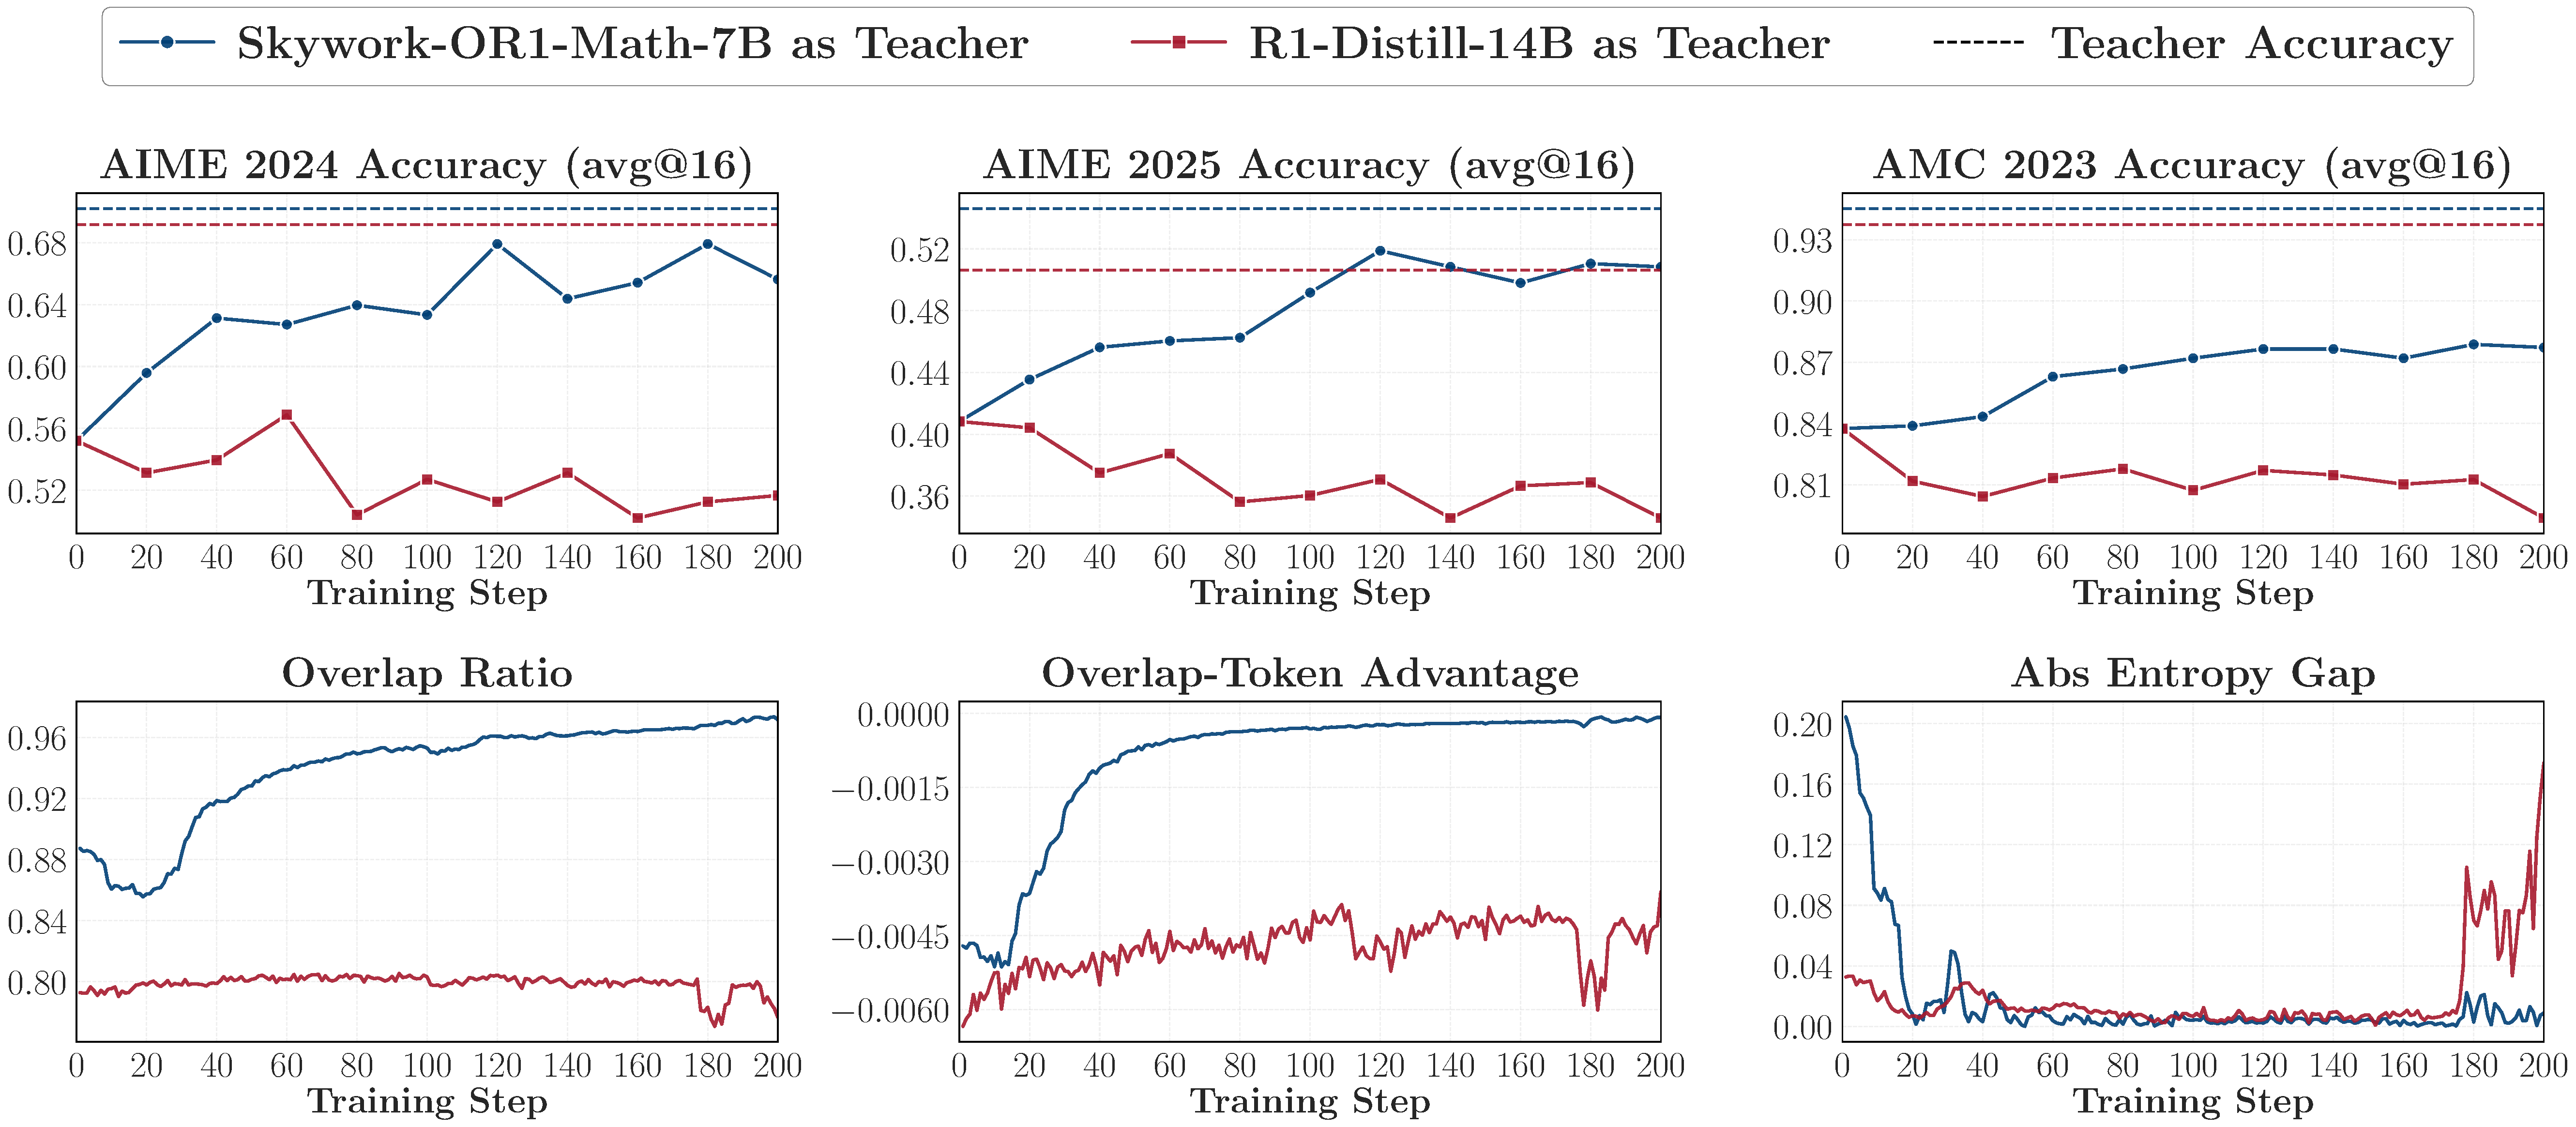
\includegraphics[width=\textwidth]{Figures/appendix/7B_setting/7B_5_1_combined.pdf}
    \caption{
    Cross-model validation with a fixed student (R1-Distill-7B) and two teachers.
    \textbf{Top:} avg@16 accuracy on AIME 2024, AIME 2025, and AMC 2023.
    \textbf{Bottom:} overlap ratio, overlap-token advantage, and absolute entropy gap over training.
    The successful run is again accompanied by increasing high-probability-token alignment, while the stagnating run is not.
    }
    \label{fig:alignment_cross_model}
\end{figure*}

\paragraph{Results.}
\Cref{fig:alignment_cross_model} shows the same pattern as \Cref{fig:alignment_main}.
With Skywork-OR1-Math-7B as the teacher, distillation improves student performance and is accompanied by steadily increasing overlap ratio, overlap-token advantage approaching zero, and a small entropy gap.
In contrast, with R1-Distill-14B as the teacher, training shows little improvement and the alignment metrics remain poor or unstable.
This provides additional evidence that successful OPD consistently coincides with the emergence of high-probability-token alignment at student-visited states.

\section{Details for \Cref{sec:recipe}}

\subsection{Cold-Start Distillation Details}
\label{app:coldstart_details}

\paragraph{Offline teacher rollout.}
To construct the cold-start SFT data, we sample 200K math prompts from the math subset of OpenThoughts3-1.2M~\citep{guha2025openthoughts} and use Qwen3-4B (Non-thinking) to generate one offline response for each prompt. For each prompt, we use the following template:
\begin{tcolorbox}[title=\textbf{Teacher rollout template}, colback=CornflowerBlue!20, colframe=CornflowerBlue!90!Black]
\small
\{Question\} Please reason step by step, and put your final answer within \textbackslash boxed\{\}.
\end{tcolorbox}
We decode with temperature $0.7$, top-$p=0.95$, top-$k=-1$, and a maximum generation length of 12{,}288 tokens. After generation, we filter out incomplete responses (e.g., truncated outputs that do not finish properly) and degenerate repetitive responses. The remaining prompt-response pairs are used as the supervised distillation corpus for training the student.

\paragraph{Student SFT.}
Starting from Qwen3-1.7B-Base, we perform full-parameter SFT on the filtered 200K teacher-generated samples using the LLaMA-Factory framework~\citep{zheng2024llamafactory}, yielding Qwen3-1.7B-SFT. We summarize the detailed hyperparameters in Table~\ref{tab:coldstart_sft_hparams}.

\begin{table}[t]
\centering
\caption{SFT hyperparameters for cold-start distillation from Qwen3-4B (Non-thinking) to Qwen3-1.7B-Base.}
\label{tab:coldstart_sft_hparams}
\begin{tabular}{ll}
\toprule
\textbf{Hyper-parameter} & \textbf{Value} \\
\midrule
Student model & Qwen3-1.7B-Base \\
Training objective & Full-parameter SFT \\
Template & \texttt{qwen3} \\
Training epochs & 1 \\
Sequence length & 14{,}336 \\
Per-device batch size & 8 \\
Gradient accumulation steps & 1 \\
Learning rate & $1 \times 10^{-5}$ \\
LR scheduler & Cosine \\
Warmup ratio & 0.05 \\
Precision & BF16 \\
\bottomrule
\end{tabular}
\end{table}

\subsection{Additional Analysis of Overlap Mass}
\label{app:add_analysis_of_overlap_mass}

To better understand why the base-initialized student can occasionally exhibit a comparable or even slightly better Overlap-Token Advantage while still underperforming overall, we further examine the probability mass covered by the overlap set from both the student and teacher sides. As shown in Figure~\ref{fig:overlap_mass}, the SFT-initialized student maintains both student overlap mass and teacher overlap mass at consistently high levels throughout training. This indicates that the overlap tokens cover most of the high-probability regions of both the student and teacher distributions, suggesting a strong and stable alignment from the beginning of OPD. In contrast, the base-initialized student exhibits substantially lower and more unstable overlap mass, especially in the early stage of training. 

This analysis helps explain why Overlap-Token Advantage alone can sometimes be misleading. Since it is averaged only over overlap tokens, it can appear relatively favorable even when the overlap set itself misses substantial high-probability teacher tokens. Overlap mass complements this view by revealing whether the shared support actually covers the most important parts of the two distributions. From this perspective, the SFT cold start leads to a substantially better and more stable match between student and teacher.

\begin{figure}[t]
    \centering
    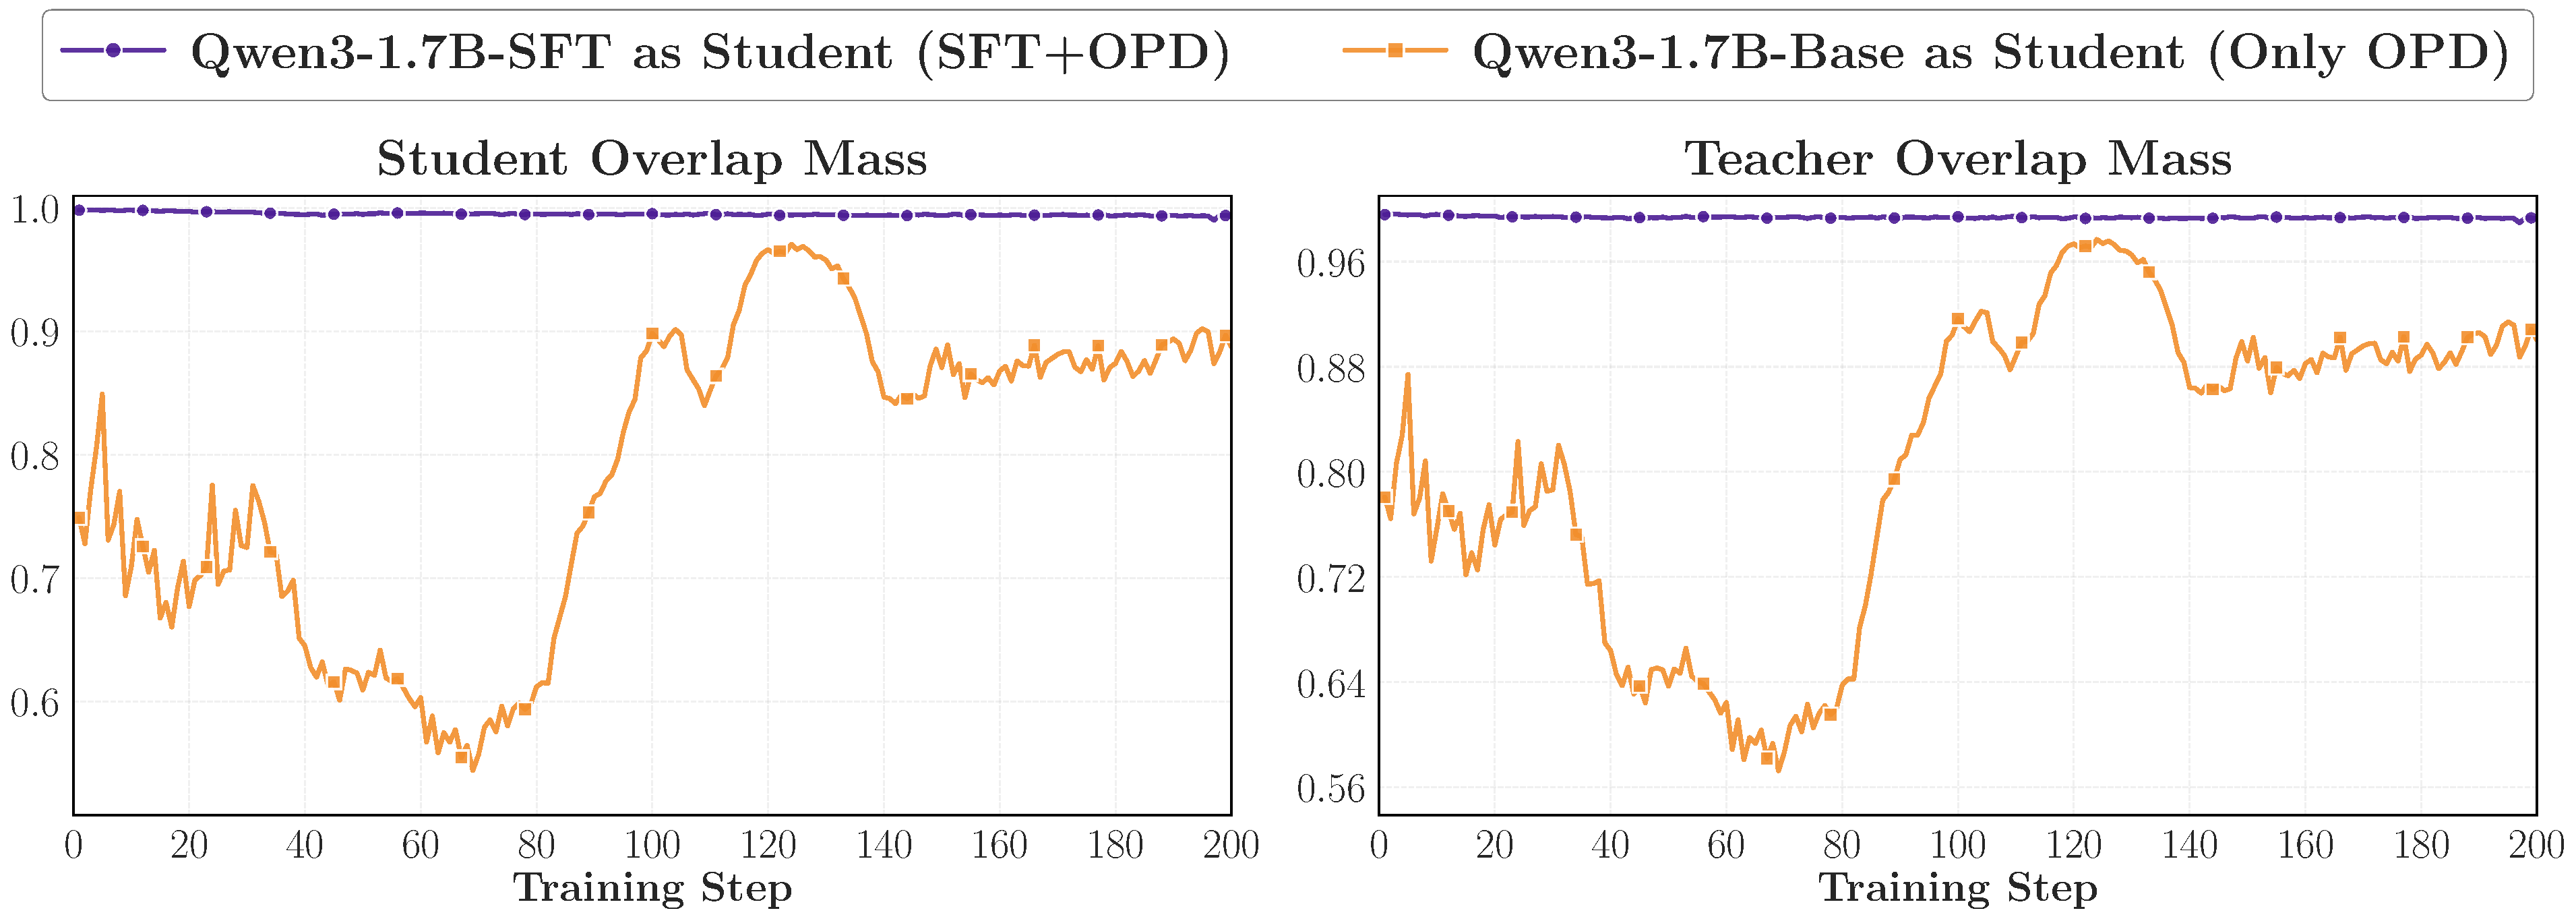
\includegraphics[width=\linewidth]{Figures/4.2/5_1_appendix_sum_p.pdf}
    \caption{Student overlap mass and teacher overlap mass during training for SFT-initialized and base-initialized students.}
    \label{fig:overlap_mass}
\end{figure}

\subsection{Deduplication Details for the DeepMath Subset}
\label{app:deepmath_dedup}

For the cross-size setting, we construct a DeepMath subset deduplicated against DAPO-Math-17K in order to compare prompts aligned with the teacher's RL post-training data against prompts that are only in-domain.

Our deduplication is performed in two stages: exact-match deduplication and semantic deduplication.

\paragraph{Question extraction.}
For both DAPO-Math-17K and DeepMath, we extract the question content and remove the instruction suffix in the prompt, so that deduplication is performed based on the question text alone.

\paragraph{Stage 1: Exact-match deduplication.}
We collect all extracted DAPO-Math-17K questions into a set and remove any DeepMath example whose extracted question exactly matches one of the DAPO questions.

\paragraph{Stage 2: Semantic deduplication.}
To further remove near-duplicate prompts, we encode both DAPO-Math-17K and DeepMath questions using the sentence embedding model all-mpnet-base-v2~\citep{reimers2019sentencebert}.
We L2-normalize the embeddings and build a FAISS inner-product index over the DAPO embeddings, so that the inner product corresponds to cosine similarity.
For each DeepMath question, we retrieve its top-1 nearest neighbor in DAPO-Math-17K.
If the cosine similarity to the nearest DAPO question is at least $0.6$, we mark the DeepMath example as a semantic duplicate and remove it.

\paragraph{Final retained subset.}
We remove any DeepMath example flagged by either exact-match or semantic deduplication.
The resulting subset is in-domain but deduplicated against DAPO-Math-17K, enabling a controlled comparison between prompts that overlap with the teacher's post-training data and prompts that are only in-domain.










\begin{figure*}[t]
    \centering
    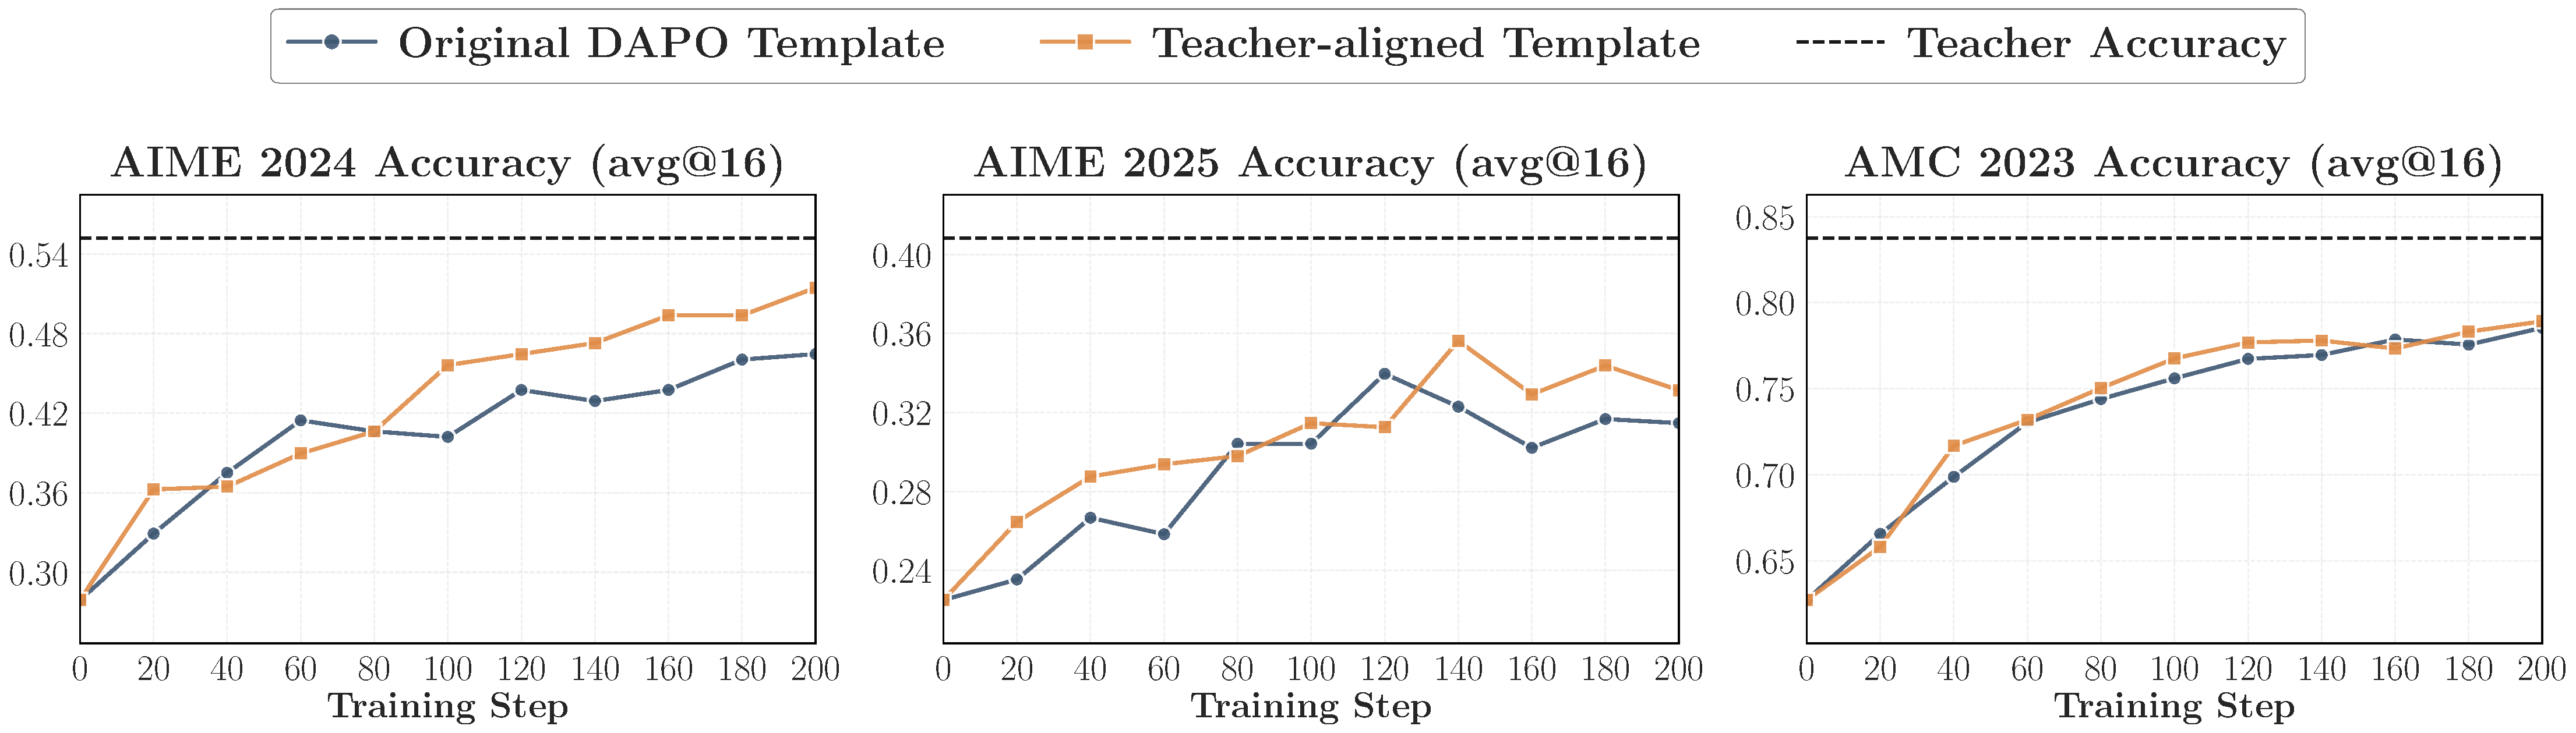
\includegraphics[width=\textwidth]{Figures/4.3/4_3_Same_benchmarks.pdf}
    \caption{Benchmark-wise breakdown of the average validation accuracy shown in \Cref{fig:teacher_posttrain_data_same}. Using the teacher-aligned template consistently matches or outperforms the original DAPO template across the three benchmarks.}
    \label{fig:teacher_posttrain_data_same_breakdown}
\end{figure*}


\subsection{Benchmark-wise breakdown of prompt-template alignment}
\label{app:teacher_template_breakdown}

To further unpack the averaged result in \Cref{fig:teacher_posttrain_data_same}, \Cref{fig:teacher_posttrain_data_same_breakdown} presents a benchmark-wise breakdown.
The teacher-aligned template yields broadly consistent improvements across datasets, with larger gains on the two AIME sets and a smaller but still positive effect on AMC 2023.
It also allows the student to recover a larger fraction of the teacher's performance, increasing from roughly 80\% to roughly 85\%.
Together with the overlap-ratio result in \Cref{sec:teacher_posttrain_data}, this suggests that prompt-template alignment improves OPD by making the student's generated states more compatible with the teacher.



\section{Details for \Cref{sec:discussion}}

\subsection{Teacher entropy by output position}
\label{appendix:teacher_entropy_by_position}

To complement the student entropy analysis in \Cref{sec:reward_noise}, we also visualize teacher entropy as a function of output position across training steps under the 15$K$ max response length setting (see \Cref{fig:teacher_entropy_by_position_appendix}). Similar to the student, teacher entropy first increases at later decoding positions and then progressively propagates toward earlier tokens over training.

\begin{figure*}[t]
    \centering
    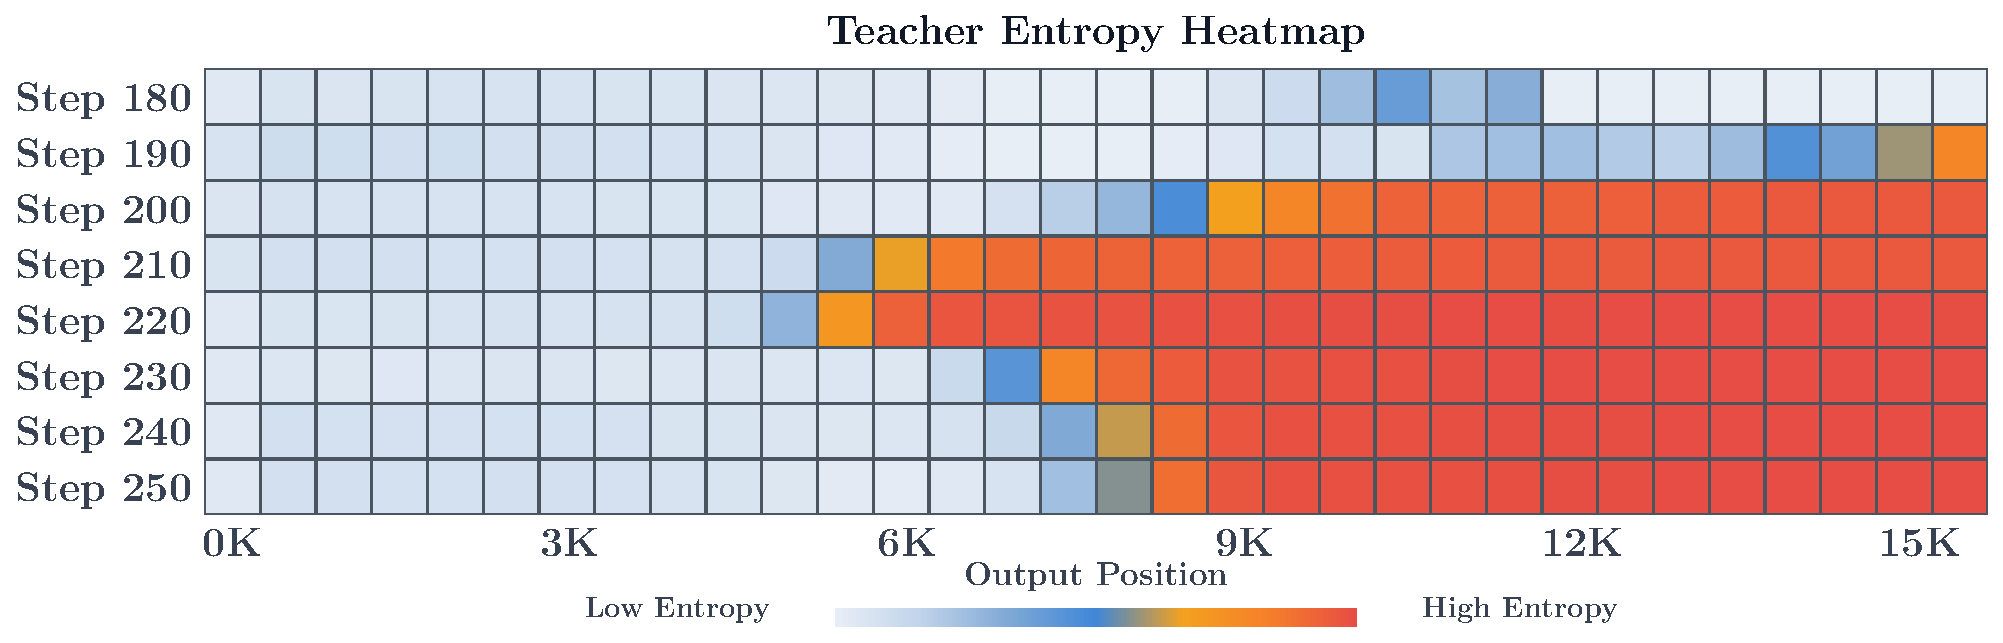
\includegraphics[width=\textwidth]{Figures/4.1/4.1.4/teacher_entropy_heatmap.pdf}
    \caption{
    Average teacher entropy across decoding positions during OPD training with 15K max response length, measured on student-generated trajectories from Step 180 to Step 250. Elevated entropy first emerges in the suffix and gradually propagates toward earlier output positions over training.
    }
    \label{fig:teacher_entropy_by_position_appendix}
\end{figure*}






